\chapter{Gráficos do Experimento 3}
\subsubsection{Algoritmo Genético Geracional Clásico}
As Figuras \ref{fig:graphGC3-01}-\ref{fig:graphGC3-10} apresentam a evolução do VPL da melhor solução, da pior solução e a média da população das dez execuções do Algoritmo Genético Geracional Clássico durante o Experimento 3 da Etapa 1 ($AG^{CC-3}$).

\begin{figure}[H]
\centering
\includegraphics[scale=1]{apxC/aggc/1}
\caption{Primeira execução da versão clássica Algoritmo Genético Geracional com 100 indivíduos na população.}
\label{fig:graphGC3-01}
\end{figure}

\begin{figure}[H]
\centering
\includegraphics[scale=1]{apxC/aggc/2}
\caption{Segunda execução da versão clássica Algoritmo Genético Geracional com 100 indivíduos na população.}
\label{fig:graphGC3-02}
\end{figure}

\begin{figure}[H]
\centering
\includegraphics[scale=1]{apxC/aggc/3}
\caption{Terceira execução da versão clássica Algoritmo Genético Geracional com 100 indivíduos na população.}
\label{fig:graphGC3-03}
\end{figure}

\begin{figure}[H]
\centering
\includegraphics[scale=1]{apxC/aggc/4}
\caption{Quarta execução da versão clássica Algoritmo Genético Geracional com 100 indivíduos na população.}
\label{fig:graphGC3-01}
\end{figure}

\begin{figure}[H]
\centering
\includegraphics[scale=1]{apxC/aggc/5}
\caption{Quinta execução da versão clássica Algoritmo Genético Geracional com 100 indivíduos na população.}
\label{fig:graphGC3-05}
\end{figure}

\begin{figure}[H]
\centering
\includegraphics[scale=1]{apxC/aggc/6}
\caption{Sexta execução da versão clássica Algoritmo Genético Geracional com 100 indivíduos na população.}
\label{fig:graphGC3-06}
\end{figure}

\begin{figure}[H]
\centering
\includegraphics[scale=1]{apxC/aggc/7}
\caption{Sétima execução da versão clássica Algoritmo Genético Geracional com 100 indivíduos na população.}
\label{fig:graphGC3-07}
\end{figure}

\begin{figure}[H]
\centering
\includegraphics[scale=1]{apxC/aggc/8}
\caption{Oitava execução da versão clássica Algoritmo Genético Geracional com 100 indivíduos na população.}
\label{fig:graphGC3-08}
\end{figure}

\begin{figure}[H]
\centering
\includegraphics[scale=1]{apxC/aggc/9}
\caption{Nona execução da versão clássica Algoritmo Genético Geracional com 100 indivíduos na população.}
\label{fig:graphGC3-09}
\end{figure}

\begin{figure}[H]
\centering
\includegraphics[scale=1]{apxC/aggc/10}
\caption{Décima execução da versão clássica Algoritmo Genético Geracional com 100 indivíduos na população.}
\label{fig:graphGC3-10}
\end{figure}

As Figuras \ref{fig:graphGC3-01}-\ref{fig:graphGC3-10} apresentam a evolução do VPL da melhor solução, da pior solução e a média da população das dez execuções do Algoritmo Genético de Regime Permanente durante o Experimento 3 da Etapa 1 ($AG^{CC-3}$).

\begin{figure}[H]
\centering
\includegraphics[scale=1]{apxC/agrpc/1}
\caption{Primeira execução da versão clássica Algoritmo de Regime Permanente com 100 indivíduos na população.}
\label{fig:graphRPC3-01}
\end{figure}

\begin{figure}[H]
\centering

\includegraphics[scale=1]{apxC/agrpc/2}

\end{figure}
\begin{figure}[H]
\centering

\includegraphics[scale=1]{apxC/agrpc/3}

\end{figure}
\begin{figure}[H]
\centering

\includegraphics[scale=1]{apxC/agrpc/4}

\end{figure}
\begin{figure}[H]
\centering

\includegraphics[scale=1]{apxC/agrpc/5}

\end{figure}
\begin{figure}[H]
\centering

\includegraphics[scale=1]{apxC/agrpc/6}

\end{figure}
\begin{figure}[H]
\centering

\includegraphics[scale=1]{apxC/agrpc/7}

\end{figure}
\begin{figure}[H]
\centering

\includegraphics[scale=1]{apxC/agrpc/8}

\end{figure}
\begin{figure}[H]
\centering

\includegraphics[scale=1]{apxC/agrpc/9}

\end{figure}
\begin{figure}[H]
\centering

\includegraphics[scale=1]{apxC/agrpc/10}

\end{figure}